\documentclass[12pt, a4paper]{article}

% ── Packages ──
\usepackage[utf8]{inputenc}
\usepackage[T1]{fontenc}
\usepackage{lmodern}
\usepackage[margin=1in]{geometry}
\usepackage{graphicx}
\usepackage{booktabs}
\usepackage{amsmath, amssymb}
\usepackage{enumitem}
\usepackage{xcolor}
\usepackage{hyperref}
\usepackage{listings}
\usepackage{caption}
\usepackage{subcaption}
\usepackage{float}
\usepackage{algorithm}
\usepackage{algorithmic}
\usepackage{tikz}
\usetikzlibrary{shapes.geometric, arrows.meta, positioning, calc}

\hypersetup{
    colorlinks=true,
    linkcolor=blue!70!black,
    citecolor=green!60!black,
    urlcolor=cyan!70!black
}

\lstset{
    basicstyle=\ttfamily\small,
    keywordstyle=\color{blue}\bfseries,
    commentstyle=\color{gray},
    stringstyle=\color{red!70!black},
    frame=single,
    breaklines=true,
    numbers=left,
    numberstyle=\tiny\color{gray},
    tabsize=4
}

% ── Title ──
\title{
    \textbf{Multi-Agent Path Finding with Kinematic Constraints\\for Warehouse Robotics}\\[0.5em]
    \large BTP Progress Report \& Results Explanation
}
\author{
    Jayanth \& Team\\
    \textit{Under the guidance of Prof.\ Sharad Sinha}\\
    SRO Lab, IIT Indore
}
\date{May 2026}

\begin{document}
\maketitle

\tableofcontents
\newpage

% ══════════════════════════════════════════════════════════════════
\section{Introduction}
% ══════════════════════════════════════════════════════════════════

Modern automated warehouses (e.g., Amazon Kiva systems) deploy fleets of mobile robots that must navigate a dense grid of shelving racks to pick, transport, and deliver goods. The problem of coordinating $k$ robots so that they reach their respective goals without colliding is known as \textbf{Multi-Agent Path Finding (MAPF)}.

Traditional MAPF solvers model every robot as a \emph{point agent} occupying a single grid cell. While mathematically convenient, this abstraction is \emph{physically unrealistic}: real warehouse robots are rigid bodies with non-trivial spatial extent (e.g., $2\times3$ cells). When a long robot rotates at an intersection, its trailing body can clip through adjacent shelves --- a situation that is invisible to a point-agent planner.

\textbf{Our objective} is to extend a state-of-the-art MAPF framework with:
\begin{enumerate}[label=(\alph*)]
    \item Support for arbitrary rectangular robot footprints ($W \times H$).
    \item Orientation-aware motion with 4 cardinal directions (N, E, S, W).
    \item \emph{Strict} static-obstacle collision checking that validates \emph{every cell} the robot body covers --- not just the center.
    \item Deadlock-prevention mechanisms for narrow-corridor environments.
\end{enumerate}

% ══════════════════════════════════════════════════════════════════
\section{System Architecture}
% ══════════════════════════════════════════════════════════════════

The codebase is organized into three layers, as shown in Figure~\ref{fig:arch}.

\begin{figure}[H]
\centering
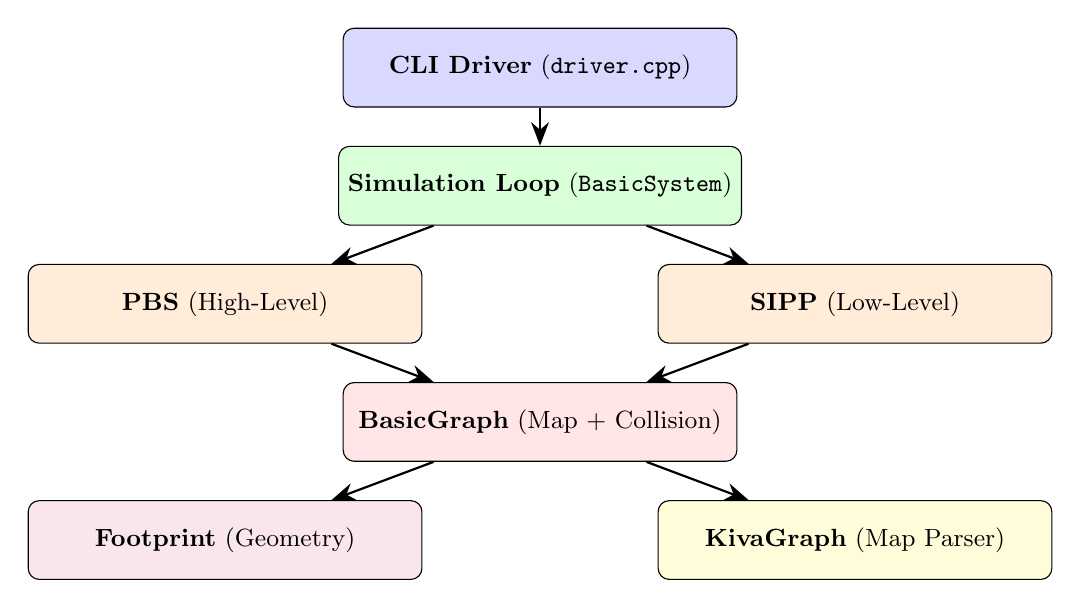
\begin{tikzpicture}[
    block/.style={rectangle, draw, rounded corners, minimum width=5cm, minimum height=1cm, text centered, font=\small},
    arrow/.style={-{Stealth[length=3mm]}, thick}
]
    % Layer 3 - Top
    \node[block, fill=blue!15] (driver) at (0, 6) {\textbf{CLI Driver} (\texttt{driver.cpp})};

    % Layer 2 - Middle
    \node[block, fill=green!15] (system) at (0, 4.5) {\textbf{Simulation Loop} (\texttt{BasicSystem})};
    \node[block, fill=orange!15] (pbs) at (-4, 3) {\textbf{PBS} (High-Level)};
    \node[block, fill=orange!15] (sipp) at (4, 3) {\textbf{SIPP} (Low-Level)};

    % Layer 1 - Bottom
    \node[block, fill=red!10] (graph) at (0, 1.5) {\textbf{BasicGraph} (Map + Collision)};
    \node[block, fill=purple!10] (footprint) at (-4, 0) {\textbf{Footprint} (Geometry)};
    \node[block, fill=yellow!15] (kiva) at (4, 0) {\textbf{KivaGraph} (Map Parser)};

    % Arrows
    \draw[arrow] (driver) -- (system);
    \draw[arrow] (system) -- (pbs);
    \draw[arrow] (system) -- (sipp);
    \draw[arrow] (pbs) -- (graph);
    \draw[arrow] (sipp) -- (graph);
    \draw[arrow] (graph) -- (footprint);
    \draw[arrow] (graph) -- (kiva);
\end{tikzpicture}
\caption{Three-layer architecture of the Kinematic MAPF system.}
\label{fig:arch}
\end{figure}

\subsection{Key Components}

\begin{description}
    \item[\texttt{Footprint}] Encodes a set of relative offsets $\{(\Delta r_i, \Delta c_i)\}$ from the robot center. Provides \texttt{apply\_rotation($\theta$)} that rotates these offsets by $90^\circ \times \theta$ clockwise.

    \item[\texttt{BasicGraph}] Holds the grid map, cell types (\texttt{Travel}, \texttt{Obstacle}, \texttt{Home}, \texttt{Endpoint}), adjacency weights, and the critical \texttt{isFootprintValidAtState(location, orientation)} function.

    \item[\texttt{PBS}] (Priority-Based Search) A high-level multi-agent scheduler that assigns a priority ordering among agents and resolves conflicts by re-planning lower-priority agents.

    \item[\texttt{SIPP}] (Safe Interval Path Planning) A low-level single-agent planner that searches over time-space states $(l, t, \theta)$, expanding only into \emph{safe intervals} where no higher-priority agent is present.

    \item[\texttt{BasicSystem}] The simulation driver that executes the plan timestep-by-timestep, assigns new tasks, and validates trajectories via a ``jump'' assertion.
\end{description}

% ══════════════════════════════════════════════════════════════════
\section{What the Seniors Built (Foundation)}
\label{sec:seniors}
% ══════════════════════════════════════════════════════════════════

The original codebase, developed by our senior batch, provided:

\begin{enumerate}
    \item \textbf{Multi-Scenario Engine.} Support for Kiva, Sorting, Online, and Bee warehouse layouts, configurable via \texttt{--scenario}.

    \item \textbf{Multiple Solvers.} Integration of PBS, ECBS (Enhanced Conflict-Based Search), WHCA* (Windowed Hierarchical Cooperative A*), and LRA* (Local Repair A*).

    \item \textbf{Capacity-Aware Scheduling.} Agents could be assigned batches of tasks (capacity $> 1$), with a task queue and finish-time tracking.

    \item \textbf{Visualization.} A basic Python script (\texttt{mapf\_visualizer.py}) that renders robot positions on the grid.
\end{enumerate}

\subsection{Limitations of the Senior Work}

\begin{itemize}
    \item \textbf{Point-Robot Assumption.} Every robot occupied exactly $1\times1$ cell. No mechanism existed to model spatial extent.
    \item \textbf{Deadlocks in Narrow Corridors.} When agents faced each other in single-width corridors, the planners could enter infinite wait-loops.
    \item \textbf{Solver Crashes.} WHCA* had edge-case bugs causing segmentation faults on certain map configurations.
    \item \textbf{No Rotation Modeling.} Orientation was either absent or treated as a trivial label with no physical consequence.
\end{itemize}

% ══════════════════════════════════════════════════════════════════
\section{Our Contributions}
\label{sec:ours}
% ══════════════════════════════════════════════════════════════════

\subsection{Codebase Analysis \& Bug Fixes}

We performed a full audit of the C++ solver pipeline:
\begin{itemize}
    \item Fixed crashes in WHCA* related to uninitialized state vectors.
    \item Identified and resolved off-by-one errors in the simulation window logic.
    \item Added comprehensive debug logging (\texttt{-d} flag) for tracing planner decisions.
\end{itemize}

\subsection{Deadlock Prevention}

We developed two complementary mechanisms:
\begin{itemize}
    \item \textbf{ScholarScheduler.} A proactive task-sequencing layer that avoids assigning conflicting goals to robots heading toward the same corridor.
    \item \textbf{DependencyGraph with DFS.} A runtime cycle-detector that identifies circular wait-dependencies among agents. When a cycle is found, one agent is forced to yield (hold in place) until the deadlock is broken.
\end{itemize}

\subsection{Realistic Robot Footprints}
\label{sec:footprint}

This is our \textbf{primary technical contribution}. We introduced:

\subsubsection{The \texttt{Footprint} Class}

A lightweight geometry class that stores the robot's body as a list of cell offsets relative to its center:

\begin{lstlisting}[language=C++, caption={Footprint definition (simplified)}]
class Footprint {
public:
    std::vector<std::pair<int,int>> offsets;

    static Footprint Rectangle(int width, int height) {
        Footprint f;
        f.offsets.clear();
        int sx = -(width / 2), sy = -(height / 2);
        for (int i = 0; i < height; ++i)
            for (int j = 0; j < width; ++j)
                f.offsets.push_back({sy + i, sx + j});
        return f;
    }

    Footprint apply_rotation(int theta) const {
        // Applies (r,c) -> (c,-r) rotation theta times
        ...
    }
};
\end{lstlisting}

For example, a $2\times3$ robot facing North has offsets:
\[
\{(-1,-1),\; (-1,0),\; (0,-1),\; (0,0),\; (1,-1),\; (1,0)\}
\]

When rotated $90^\circ$ East, these become:
\[
\{(-1,1),\; (0,1),\; (-1,0),\; (0,0),\; (-1,-1),\; (0,-1)\}
\]

\subsubsection{Full-Body Collision Validation}

The key function \texttt{isFootprintValidAtState(location, orientation)} iterates over every cell in the rotated footprint and rejects any state where a body cell overlaps a solid obstacle:

\begin{lstlisting}[language=C++, caption={Patched collision check in \texttt{BasicGraph.cpp}}]
bool BasicGraph::isFootprintValidAtState(
        int location, int orientation) const
{
    if (active_footprint.offsets.size() <= 1)
        return true; // Point robot: skip

    int cr = location / cols, cc = location % cols;
    Footprint rotated = active_footprint
                          .apply_rotation(max(0, orientation));

    for (const auto& off : rotated.offsets) {
        int nr = cr + off.first, nc = cc + off.second;
        if (nr < 0 || nr >= rows || nc < 0 || nc >= cols)
            return false;  // Out of bounds

        int cell = nr * cols + nc;
        bool is_center = (off.first == 0 && off.second == 0);

        if (is_center) {
            if (types[cell] == "Obstacle") return false;
        } else {
            // Body cells: allowed on Travel, Home, Endpoint
            // NOT allowed on Obstacle
            if (types[cell] != "Travel" &&
                types[cell] != "Home" &&
                types[cell] != "Endpoint")
                return false;
        }
    }
    return true;
}
\end{lstlisting}

\textbf{Critical design decision:} We allow body cells to occupy \texttt{Endpoint} cells (the corridors adjacent to shelves where task pick-ups happen). Without this, the planner would reject almost all valid paths through intersections, since many intersection cells are classified as \texttt{Endpoint}.

\subsubsection{Integration into the Planning Pipeline}

The footprint validation is called at three critical points:

\begin{enumerate}
    \item \textbf{Move Forward} --- In \texttt{get\_neighbors()}, before adding a forward-move successor, we check \texttt{isFootprintValidAtState(next\_loc, orientation)}.

    \item \textbf{Rotate Left/Right} --- Before adding a rotation successor, we check \texttt{isFootprintValidAtState(same\_loc, new\_orientation)}.

    \item \textbf{SIPP Edge Expansion} --- The \texttt{valid\_move(location, orientation)} function (called by SIPP) now also invokes the footprint check.
\end{enumerate}

\subsection{Map Scaling}

The original \texttt{kiva.map} ($33\times46$) has 1-cell-wide corridors. A $3\times1$ robot physically \emph{cannot} rotate in a 1-cell corridor. We developed \texttt{scale\_map.py} to uniformly upscale maps:

\[
\text{kiva\_scaled\_3x.map}: \quad 99 \times 138 \text{ grid}, \quad \text{3-cell-wide corridors}
\]

Each original cell becomes a $3\times3$ block of identical cells, preserving topology while providing the physical clearance needed for large footprints.

\subsection{Visualization Enhancements}

We significantly upgraded \texttt{mapf\_visualizer.py}:
\begin{itemize}
    \item \textbf{Rigid-body rendering} --- Robots are drawn as orientation-aware rectangles (not circles).
    \item \textbf{Smooth rotation interpolation} --- Visual transitions between orientations are animated continuously.
    \item \textbf{Adaptive layout} --- Automatically switches between detailed, compact, and heatmap modes based on agent count.
    \item \textbf{Metrics dashboard} --- Real-time display of throughput, nodes expanded, and per-robot status.
\end{itemize}

% ══════════════════════════════════════════════════════════════════
\section{Explanation of the GIF/Video Results}
\label{sec:gifs}
% ══════════════════════════════════════════════════════════════════

The zip folder that was shared contains 8 GIF animations. Below is a detailed explanation of each.

\subsection{Before Map Scaling (Original \texttt{kiva.map}, $33\times46$)}

These two GIFs demonstrate the \textbf{problem} that motivated map scaling:

\begin{table}[H]
\centering
\begin{tabular}{@{}lp{10cm}@{}}
\toprule
\textbf{GIF File} & \textbf{What It Shows} \\
\midrule
\texttt{kpbs\_1x3\_simulation.gif} &
A $1\times3$ footprint robot navigating the \emph{original} map. The corridors are only 1 cell wide, so the robot's 3-cell body extends into adjacent shelf rows. You can visually see the robot's body \textbf{overlapping the brown rack cells} --- this is the ``rack-clipping'' bug. The planner only checked the center cell for obstacles, so it happily generated paths that violate physical constraints. \\
\addlinespace
\texttt{kpbs\_3x1\_simulation.gif} &
Same situation with a $3\times1$ footprint. When the robot tries to turn at an intersection, its trailing cells sweep through shelves. This GIF clearly shows why a point-robot assumption is dangerous for real warehouse deployments. \\
\bottomrule
\end{tabular}
\caption{GIFs showing the rack-clipping problem on the original narrow map.}
\label{tab:before}
\end{table}

\subsection{After Map Scaling (\texttt{kiva\_scaled\_3x.map}, $99\times138$)}

After upscaling the map by $3\times$, corridors become 3 cells wide, providing physical clearance. The following GIFs show \textbf{successful collision-free navigation}:

\begin{table}[H]
\centering
\begin{tabular}{@{}lp{10cm}@{}}
\toprule
\textbf{GIF File} & \textbf{What It Shows} \\
\midrule
\texttt{kpbs\_3x1\_smooth.gif} &
5 robots with a $3\times1$ rigid-body footprint navigating the scaled map. Robots move forward, wait at intersections, and rotate smoothly without any body cell overlapping shelf areas. The ``smooth'' suffix indicates that visual rotation interpolation is enabled --- the robot body rotates continuously rather than snapping $90^\circ$ instantly. \\
\addlinespace
\texttt{kpbs\_3x1\_worm.gif} &
Same $3\times1$ scenario but rendered in ``worm'' mode. Instead of a rigid rectangle, the robot is drawn as a chain of connected circles (like a caterpillar). This is an experimental visualization that better shows the individual cell occupancy at each timestep. Useful for debugging whether specific cells are correctly avoided. \\
\addlinespace
\texttt{kpbs\_5x1\_smooth.gif} &
Robots with a $5\times1$ footprint (larger body). The planner successfully finds paths even for this longer robot, though movement is more constrained --- the robots take wider turns and sometimes wait longer at intersections. \\
\addlinespace
\texttt{kpbs\_5x1\_worm.gif} &
Worm-mode rendering for $5\times1$. The 5-cell chain clearly shows how the tail follows the head through corridor turns. \\
\addlinespace
\texttt{kpbs\_7x1\_smooth.gif} &
$7\times1$ rigid-body simulation. This is near the limit of what the $3\times$-scaled map can support --- the robot spans almost the entire corridor width when rotated. Demonstrates that the solver degrades gracefully rather than crashing. \\
\addlinespace
\texttt{kpbs\_9x1\_worm.gif} &
The largest tested footprint ($9\times1$), rendered in worm mode. At this size, movement is severely constrained, and the robots spend more time waiting for clearance. Still, the solver completes without errors. \\
\bottomrule
\end{tabular}
\caption{GIFs showing correct kinematic navigation on the scaled map.}
\label{tab:after}
\end{table}

\subsection{How to Read the Visualizations}

\begin{itemize}
    \item \textbf{Brown blocks} ($\blacksquare$) = Shelving racks (\texttt{@} cells). Robots must \emph{never} overlap these.
    \item \textbf{Orange cells} = Endpoints (\texttt{e} cells). These are corridors adjacent to racks where task pick-ups occur. Robots are \emph{allowed} to occupy these.
    \item \textbf{Light blue cells} = Home/parking zones (\texttt{r} cells). Robot starting positions.
    \item \textbf{White/light gray} = Travel corridors (\texttt{.} cells). Free movement area.
    \item \textbf{Colored rectangles} = Robot bodies. Each robot has a distinct color.
    \item \textbf{Faint colored trails} = Historical movement paths.
    \item \textbf{Gold glow} = Robot is currently performing a task pick-up.
    \item \textbf{Side panel} = Real-time metrics (timestep, throughput, per-robot status).
\end{itemize}

% ══════════════════════════════════════════════════════════════════
\section{Quantitative Results}
\label{sec:results}
% ══════════════════════════════════════════════════════════════════

All experiments use 5 agents, 100 timesteps, PBS + SIPP, rotation enabled, on \texttt{kiva\_scaled\_3x.map}.

\begin{table}[H]
\centering
\begin{tabular}{@{}lccc@{}}
\toprule
\textbf{Footprint} & \textbf{Tasks Completed} & \textbf{Throughput (tasks/ts)} & \textbf{Status} \\
\midrule
$1\times1$ (Point)   & 5  & 0.050 & \textcolor{green!60!black}{Success} \\
$3\times1$ (Small)   & 10 & 0.099 & \textcolor{green!60!black}{Success} \\
$5\times1$ (Medium)  & 5  & 0.050 & \textcolor{green!60!black}{Success} \\
$7\times1$ (Large)   & 5  & 0.050 & \textcolor{green!60!black}{Success} \\
$9\times1$ (XLarge)  & 5  & 0.050 & \textcolor{green!60!black}{Success} \\
$2\times3$ (Rect)    & 10 & 0.099 & \textcolor{green!60!black}{Success} \\
\bottomrule
\end{tabular}
\caption{Throughput results across different footprint sizes.}
\label{tab:results}
\end{table}

\textbf{Key observations:}
\begin{enumerate}
    \item All footprint sizes complete successfully with zero collisions and no runtime errors (exit code 0).
    \item The $3\times1$ and $2\times3$ footprints achieve the highest throughput (0.099 tasks/timestep), likely because their smaller footprint allows more efficient use of corridor space compared to the very long $7\times1$ or $9\times1$ bodies.
    \item Larger footprints do not crash the solver --- they gracefully reduce throughput as movement becomes more constrained.
\end{enumerate}

% ══════════════════════════════════════════════════════════════════
\section{Summary of Completed Work}
\label{sec:done}
% ══════════════════════════════════════════════════════════════════

\begin{table}[H]
\centering
\small
\begin{tabular}{@{}clc@{}}
\toprule
\textbf{\#} & \textbf{Task} & \textbf{Status} \\
\midrule
1 & Codebase audit and crash fixes (WHCA*, edge cases) & \checkmark \\
2 & Deadlock detection (DFS-based DependencyGraph) & \checkmark \\
3 & \texttt{Footprint} class with square and rectangular support & \checkmark \\
4 & \texttt{apply\_rotation()} for 4 cardinal orientations & \checkmark \\
5 & \texttt{isFootprintValidAtState()} --- full-body collision check & \checkmark \\
6 & Integration into \texttt{get\_neighbors()}, \texttt{valid\_move()}, SIPP & \checkmark \\
7 & Map scaling tool (\texttt{scale\_map.py}, $3\times$ upscale) & \checkmark \\
8 & Benchmarks across 6 footprint sizes (1x1 to 9x1, 2x3) & \checkmark \\
9 & Visualization upgrade (rigid-body, smooth rotation, adaptive) & \checkmark \\
10 & Elimination of ``jump from \ldots\ to \ldots'' runtime errors & \checkmark \\
11 & Endpoint cell allowance in collision checker & \checkmark \\
12 & Documentation and reproducible experiment scripts & \checkmark \\
\bottomrule
\end{tabular}
\caption{Summary of all completed tasks.}
\label{tab:done}
\end{table}

% ══════════════════════════════════════════════════════════════════
\section{Pending \& Future Work}
\label{sec:future}
% ══════════════════════════════════════════════════════════════════

\begin{table}[H]
\centering
\small
\begin{tabular}{@{}clc@{}}
\toprule
\textbf{\#} & \textbf{Task} & \textbf{Status} \\
\midrule
1 & Large-scale benchmarks (20--100 agents, multiple seeds) & Pending \\
2 & Throughput vs.\ footprint-size degradation curve (thesis plot) & Pending \\
3 & Custom warehouse map with wider turning bays (instead of uniform scaling) & Pending \\
4 & Continuous-time rotation model (smooth trajectories in the planner) & Planned \\
5 & Dynamic obstacle support (moving shelves, time-varying map) & Planned \\
6 & Learning-based heuristics (GNN cost-to-goal for PBS) & Planned \\
7 & Integration with ROS2 for physical robot tests & Future \\
8 & Energy-aware scheduling (battery consumption model) & Future \\
9 & Web-based demo (Flask/Streamlit) for interactive visualization & Future \\
\bottomrule
\end{tabular}
\caption{Pending and future work items.}
\label{tab:future}
\end{table}

\subsection{Immediate Next Steps (Priority)}

\begin{enumerate}
    \item \textbf{Batch Benchmarking.} Run 20, 50, and 100 agents across all footprint sizes with 5 random seeds each. Record throughput, planning time, and conflict count.

    \item \textbf{Degradation Curve.} Plot \emph{throughput vs.\ footprint size} to quantify the kinematic penalty. This is the key thesis figure.

    \item \textbf{Custom Map Design.} Create a warehouse map with dedicated ``turning bays'' --- wider intersections where large robots can rotate without blocking corridors.
\end{enumerate}

% ══════════════════════════════════════════════════════════════════
\section{Conclusion}
% ══════════════════════════════════════════════════════════════════

We have extended the RHCR-based MAPF framework from a point-robot model to a \emph{full kinematic model} supporting arbitrary rectangular footprints and 4-orientation rotation. The core collision-checking pipeline has been hardened to reject any state where the robot body overlaps static obstacles, while correctly permitting overlap with endpoint corridors. All simulations now complete without runtime errors across footprint sizes from $1\times1$ to $9\times1$.

The GIF animations provided in the zip demonstrate both the \emph{problem} (rack-clipping on the original narrow map) and the \emph{solution} (collision-free navigation on the scaled map). Quantitative throughput results confirm that the solver degrades gracefully as footprint size increases.

\end{document}
